\documentclass{article}
\usepackage[utf8]{inputenc}
\usepackage{amsmath}
\usepackage{xcolor}
\usepackage[top=2cm, bottom=2cm, left=2cm, right=2cm]{geometry}
\setlength\parindent{0pt}

\usepackage{listings}
%\usepackage{color}
\usepackage{graphicx}
\usepackage{float}
\usepackage{caption}

\usepackage{verbatim}
\let\oldv\verbatim
\let\oldendv\endverbatim

%\userpackage{minted}

\definecolor{dkgreen}{rgb}{0,0.6,0}
\definecolor{gray}{rgb}{0.5,0.5,0.5}
\definecolor{mauve}{rgb}{0.58,0,0.82}
\definecolor{light-gray}{gray}{0.95}


\lstset{frame=tb,
  language=Java,
  aboveskip=6mm,
  belowskip=6mm,
  showstringspaces=false,
  columns=flexible,
  basicstyle={\small\ttfamily},
  numbers=none,
  numberstyle=\tiny\color{gray},
  keywordstyle=\color{blue},
  commentstyle=\color{dkgreen},
  stringstyle=\color{mauve},
  breaklines=true,
  breakatwhitespace=true,
  tabsize=3,
  backgroundcolor=\color{light-gray},
  language=Matlab
}

%\usepackage{natbib} replaced by line below to make refernces work
\usepackage[square,sort,comma,numbers]{natbib}
\usepackage[nottoc,numbib]{tocbibind} %to get references in table of contants
\usepackage{graphicx}

\usepackage{bm}

\usepackage{hyperref}
\hypersetup{
	colorlinks,
	citecolor=black,
	filecolor=black,
	linkcolor=black,
	urlcolor=black
}

\usepackage{mdframed}
\usepackage{lipsum} % for creating dummy text
\mdfdefinestyle{MyFrame}{%
	linecolor=black,	
	backgroundcolor=gray!20!white,
	skipbelow = 8mm,
	skipabove = 8mm}

\usepackage{scrextend}

\usepackage{multimedia}
\usepackage{media9}

\usepackage{booktabs}

\title{Fys4150\\Project 4 Figures and stuff\\ }
\author{Peter Killingstad and Karl Jacobsen\\
\\
\url{https://github.com/kaaja/fys4150}}
\begin{document}
	
\maketitle



\section*{4b}



\begin{table}[H]
	\centering
\begin{tabular}{rrrrr}
	\hline
	mcs &      Eavg &   absMavg &        Cv &       chi \\
	\hline
	100 & -2.000000 &  1.000000 &  0.000000 &  0.000000 \\
	1000 & -1.994000 &  0.998000 &  0.047856 &  0.005984 \\
	10000 & -1.993800 &  0.997900 &  0.049446 &  0.006382 \\
	100000 & -1.995360 &  0.998450 &  0.037034 &  0.004650 \\
	1000000 & -1.995910 &  0.998620 &  0.032653 &  0.004182 \\
	10000000 & -1.995949 &  0.998646 &  0.032349 &  0.004064 \\
	100000000 & -1.995968 &  0.998656 &  0.032195 &  0.004024 \\
	1000000000 & -1.995976 &  0.998659 &  0.032133 &  0.004016 \\
	1410065408 & -1.995978 &  0.998660 &  0.032114 &  0.004011 \\
	\hline
\end{tabular}
	\caption{Estimated quantitites}
	\label{fig:4b1}
\end{table}

\begin{table}[H]
	\centering
\begin{tabular}{rrrrr}
	\hline
	mcs &      Eavg &   absMavg &          Cv &         chi \\
	\hline
	100 &  0.201300 &  0.134106 & -100.000000 & -100.000000 \\
	1000 & -0.099304 & -0.066162 &   49.166215 &   49.199418 \\
	10000 & -0.109324 & -0.076175 &   54.122962 &   59.131750 \\
	100000 & -0.031167 & -0.021102 &   15.433885 &   15.948442 \\
	1000000 & -0.003612 & -0.004079 &    1.779036 &    4.279582 \\
	10000000 & -0.001658 & -0.001435 &    0.830445 &    1.319746 \\
	100000000 & -0.000696 & -0.000456 &    0.350614 &    0.335773 \\
	1000000000 & -0.000320 & -0.000187 &    0.156479 &    0.120349 \\
	1410065408 & -0.000200 & -0.000077 &    0.097802 &    0.016475 \\
	\hline
\end{tabular}
	\caption{Percentage deviations from analytical results}
	\label{fig:4b2}
\end{table}

\section{4c}

\begin{minipage}{.45\textwidth} 
	\begin{figure}[H]
		\centering
		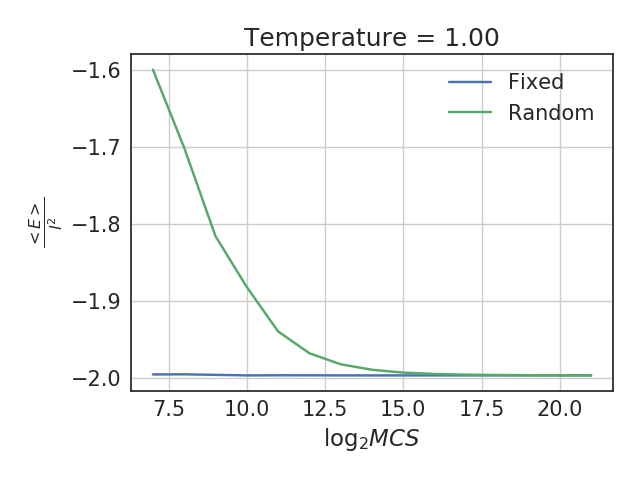
\includegraphics[width=0.99\textwidth]{/home/karl/doc/subj/att/fys4150/project4/resultsKeep/4cEnergy1.png}
		\caption{Expected Energy divided by $L^2$. $T=1.0$. \\ \textit{Equilibrium reached after $2^{20}$ Monte Carlo cycles.}}
		\label{1}
	\end{figure}
\end{minipage}\hfill
\begin{minipage}{.45\textwidth} 
	\begin{figure}[H]
		\centering
		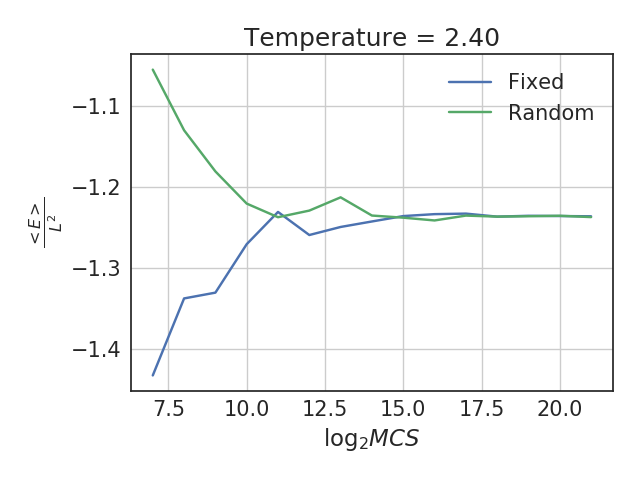
\includegraphics[width=0.99\textwidth]{/home/karl/doc/subj/att/fys4150/project4/resultsKeep/4cEnergy24.png}
		\caption{Expected Energy divided by $L^2$. $T = 2.4$. \\ \textit{Equilibrium reached at same point as for $T=1$}.}
		\label{1}
	\end{figure}
\end{minipage}\hfill
\vspace{2ex}

\begin{minipage}{.45\textwidth} 
	\begin{figure}[H]
		\centering
		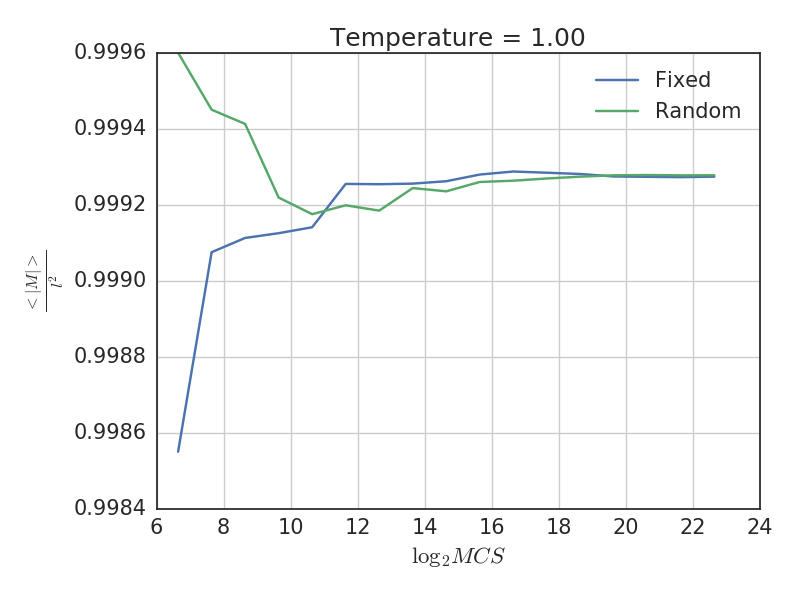
\includegraphics[width=0.99\textwidth]{/home/karl/doc/subj/att/fys4150/project4/resultsKeep/4cMoment1.png}
		\caption{Expected absolute magnetic momentum divided by $L^2$. $T = 1.0$. \\ \textit{Equilibrium reached at same point as for the energy.}}
		\label{1}
	\end{figure}
\end{minipage}\hfill
\begin{minipage}{.45\textwidth} 
	\begin{figure}[H]
		\centering
		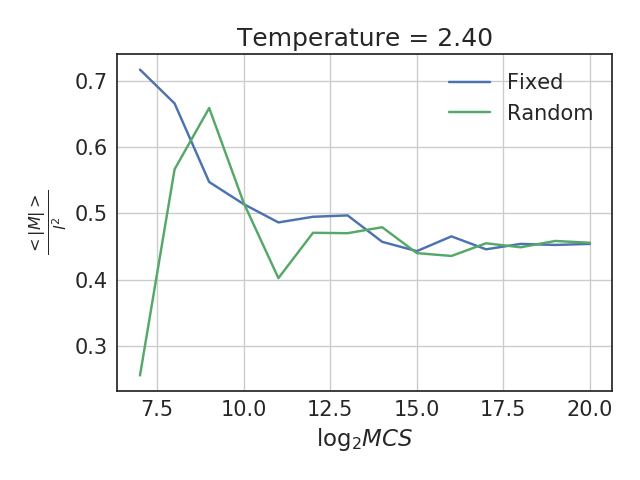
\includegraphics[width=0.99\textwidth]{/home/karl/doc/subj/att/fys4150/project4/resultsKeep/4cMoment24.png}
		\caption{Expected absolute magnetic momentum divided by $L^2$. $T = 2.4$. \\ \textit{Equilibrium reached at same point as for the others.}}
		\label{1}
	\end{figure}
\end{minipage}\hfill
\vspace{2ex}

\begin{figure}[H]
	\centering
	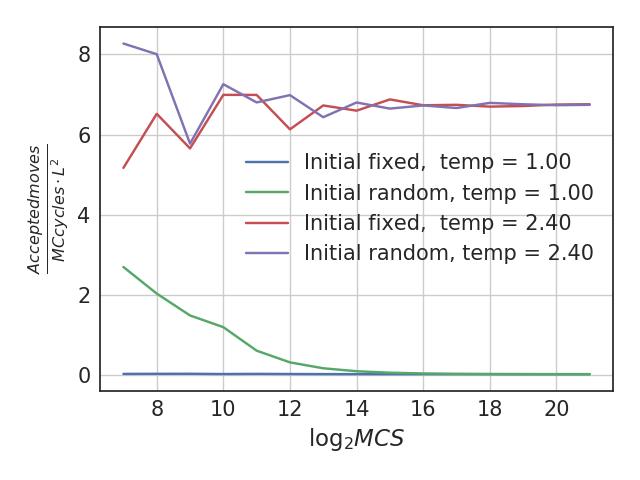
\includegraphics[width=0.6\textwidth]{/home/karl/doc/subj/att/fys4150/project4/resultsKeep/4cAcceptedMoves.png}
	\caption{Accepted moved divided by $L^2$. \\ \textit{}}
	\label{1}
\end{figure}

\section{4d}

\begin{table}[H]
	\centering
	\input{/home/karl/doc/subj/att/fys4150/project4/results/4dTableFixed.txt}%
	\caption{Statistics. Fixed initial config. 1st row $T=1$. \\ \textit{.}}
	\label{1}
\end{table}

\begin{table}[H]
	\centering
	\input{/home/karl/doc/subj/att/fys4150/project4/results/4dTableRandom.txt}%
	\caption{Statistics. Random initial config. 1st row $T=1$. \\ \textit{.}}
	\label{1}
\end{table}





\end{document}
